\documentclass[10pt, twocolumn]{jarticle}
\usepackage[caption=false]{subfig}
\usepackage{amsmath}
\usepackage{amsfonts}
\usepackage{algorithmic}
\usepackage{algorithm}
\usepackage[dvipdfmx]{graphicx}
\usepackage{bm}
\usepackage{setspace}
\usepackage{url}
\usepackage[tiny]{titlesec}

\renewcommand{\figurename}{\small 図}
\renewcommand{\tablename}{\small 表}

% 余白の上を25mm、下を20mmに
\setlength{\textheight}{\paperheight}
\addtolength{\textheight}{-45truemm}
\setlength{\topmargin}{-0.4truemm}
\addtolength{\topmargin}{-\headheight}
\addtolength{\topmargin}{-\headsep}

% 余白の左を20mm、右を20mmに
\setlength{\textwidth}{\paperwidth}
\addtolength{\textwidth}{-40truemm}
\setlength{\oddsidemargin}{-5.4truemm}

% ヘッダの設定
\usepackage{fancyhdr}
\pagestyle{fancy}
\rhead{}
\lhead{\bf 2019年度 工学部システム創成学科PSI コース 卒業論文概要}
\renewcommand{\headrulewidth}{0pt}

% 2つのカラムの間隔を設定
\setlength{\columnsep}{8mm}

% 題目の設定
\titleformat{\section}{\bf \fontsize{10pt}{12pt}}{\thesection.}{1zw}{}
\titleformat{\subsection}{\bf \fontsize{10pt}{12pt}}{\thesubsection.}{1zw}{}
\titlespacing{\section}{0pt}{*3}{*0}
\titlespacing{\subsection}{0pt}{*3}{*0}

%%%%%%%%%%%%%%%%%%%%%%%%%%%%%%%%%%%%%%%%%%%%%%%%%%
\begin{document}

\twocolumn[%
\begin{center}
{\bf \fontsize{14pt}{16pt}\selectfont 複雑環境下でのロボット学習に向けた\\深層状態空間モデルを用いた映像予測}  % 論文題目
\end{center}
\begin{flushright}
\fontsize{11pt}{13pt}\selectfont 03-180961 近藤生也\\% 学籍番号、氏名
\fontsize{11pt}{13pt}\selectfont 指導教員 松尾豊 教授% 指導教員名
\end{flushright}
]%

% 行間を0.8倍に
\setstretch{0.8}

%%%%%%%%%%%%%%%%%%%%%%%%%%%%%%%%%%%%%%%%%%%%%%%%%%
% 以下、本文
\section{序論}

近年,機械学習・深層学習を用いてロボットの制御方法をロボット自らに学ばせる{\bf ロボット学習}の研究が進んでおり,ロボットの実用化の可能性が広がっている.ロボット学習において{\bf 映像予測}は重要であり,ロボット自身の行動計画の作成や\cite{hafner2019planet},ユーザーが事前にロボットの行動を評価する際に用いることができる\cite{ebert2018visual}.映像予測のアプローチは大きく{\bf 回帰型ニューラルネットワーク}ベースの手法と{\bf 深層状態空間モデル}ベースの手法に分けられる.前者は生成精度は高いが長期の予測の際には誤差が蓄積しやすく,また予測を行うには直前までの映像を複数フレーム用意する必要があり予測してから行動したいようなロボット実機の問題設定には向いていない.一方後者は近年深層強化学習の分野で用いられており,ゲームや単純なシミュレーターを題材にした映像予測は可能なものの,複雑なデータに対してはRNNベースの手法と比較し高精度な予測が難しく,映像予測自体を目的にした研究は進んでいない.

本研究ではロボット学習への応用を前提とし,DSSMをベースにした映像予測性能の向上を目指す.提案手法として,状態表現の階層性に着目したDSSMの拡張を考え,実験によりその有効性を示す.

\section{前提知識}
\subsection{DSSM}
{\bf 深層状態空間モデル(Deep State Space Model,DSSM)}は将来の観測の予測を通して環境の状態表現を獲得する深層学習手法である\cite{krishnan2015deep}.DSSMのグラフィカルモデルは図\ref{fig:ssm}のように表され,各時刻の状態表現$s_t$の遷移とその時刻の観測$o_t$の生成過程をニューラルネットワークで表現する.DSSMは初期状態$s_0$と環境中の行動主体の行動系列$a_{1:T}$を入力とし,$o_{1:T}$を予測し出力することができる.ただし初期状態は$o_0$から求められる.

\begin{figure}[h]
  \begin{center}
    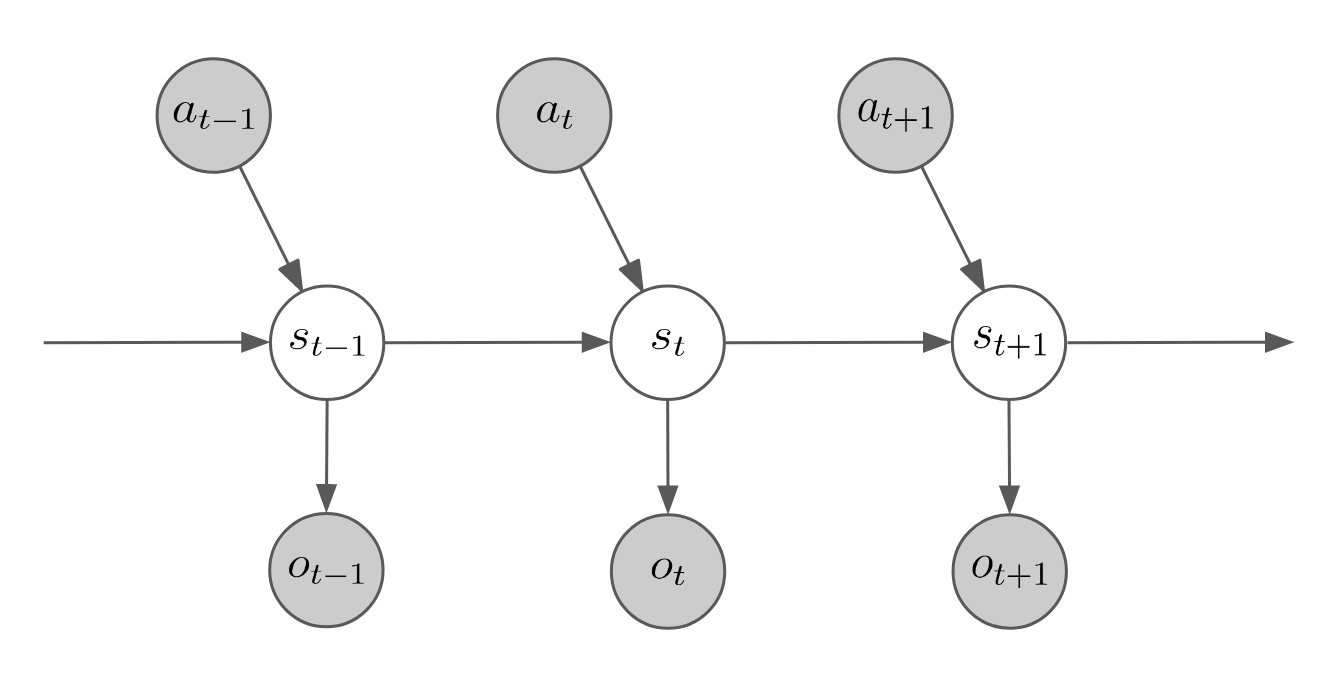
\includegraphics[width=0.8\linewidth]{./figures/dssm.png}
    \caption[DSSMのグラフィカルモデル]{\small DSSMのグラフィカルモデル.実線は生成分布,点線は推論分布を表す.簡単のため推論分布は時刻tでのみ記載している.}
    \label{fig:ssm}
  \end{center}
\end{figure}

DSSMのネットワークのパラメータは,図\ref{fig:ssm}の点線で表された推論分布$q(s_t|s_{t-1}, a_t, o_t)$を導入することで,次の変分下限の最大化によって求められる.
\small
\begin{eqnarray}
  \log p(o_{1:T}|a_{1:T}) \geq \sum_{t=1}^T ( {L}_{reconst} - {L}_{KL}) 
\end{eqnarray}
ただし,
\begin{eqnarray}
  && {L}_{reconst} = \mathbb{E}_{s_t \sim q(s_t|s_{t-1}, a_t, o_t)} [\log p(o_t|s_t)] \nonumber \\
  && {L}_{KL} = \mathbb{E}_{s_{t-1} \sim q(s_{t-1}|s_{t-2}, a_{t-1}, o_{t-1})} \nonumber \\
  && \hspace{2em} [\mathrm{D_{KL}}(q(s_t|s_{t-1}, a_t, o_t) \| p(s_t|s_{t-1}, a_t, o_t, s_t))] \hspace{6em} \nonumber
  \label{eq:dssm_elbo}  
\end{eqnarray}
\normalsize
ここで$ - L_{reconst}$は観測の再構成誤差を,$L_{KL}$は$s_t$の生成分布と近似分布の間のカルバック・ライブラー情報量を指す.
% \left( \mathbb{E}_{s_t \sim q(s_t|s_{t-1}, a_t, o_t)} [\log p(o_t|s_t)] \right. \nonumber \\
% && \hspace{2em} \left. - \mathbb{E}_{s_{t-1} \sim q(s_{t-1}|s_{t-2}, a_{t-1}, o_{t-1})} [\mathrm{D_{KL}}(q(s_t|s_{t-1}, a_t, o_t) \| p(s_t|s_{t-1}, a_t, o_t))] \right) \nonumber \\

\section{問題設定}
本研究では{\bf 行動条件付き映像予測}の問題を扱う.具体的には,行動系列と観測系列の組$\{\vec{a},\vec{o}\}$の訓練用のデータを用いて学習し,評価用のデータで初期観測$o_0$と行動系列$a_{1:10}$が与えられたときに正しく$o_{1:10}$の予測・生成ができることを目指す.本研究ではBAIR Push Dataset\cite{ebert2017selfsupervised}を用いて各手法の評価を行う.

\section{深層状態空間モデルの問題点}
予備実験としてDSSMを用いてBAIR Push Datasetで学習を行った際の学習曲線を図\ref{fig:curve}のBaseline(64) $\sim$ (1024)に示す.ただし括弧内の数字は状態変数$s_t$の次元数である.モデルが状態表現として獲得できる情報量を増やすためには素朴には状態変数の次元を大きくすることが考えるが,実際には学習がうまく進まず,性能はむしろ下がることがわかった.これを受けて潜在変数の次元を大きくした際にも学習をうまく進める方法を次のように提案する.

% \begin{figure}[h]
%   \begin{center}
%     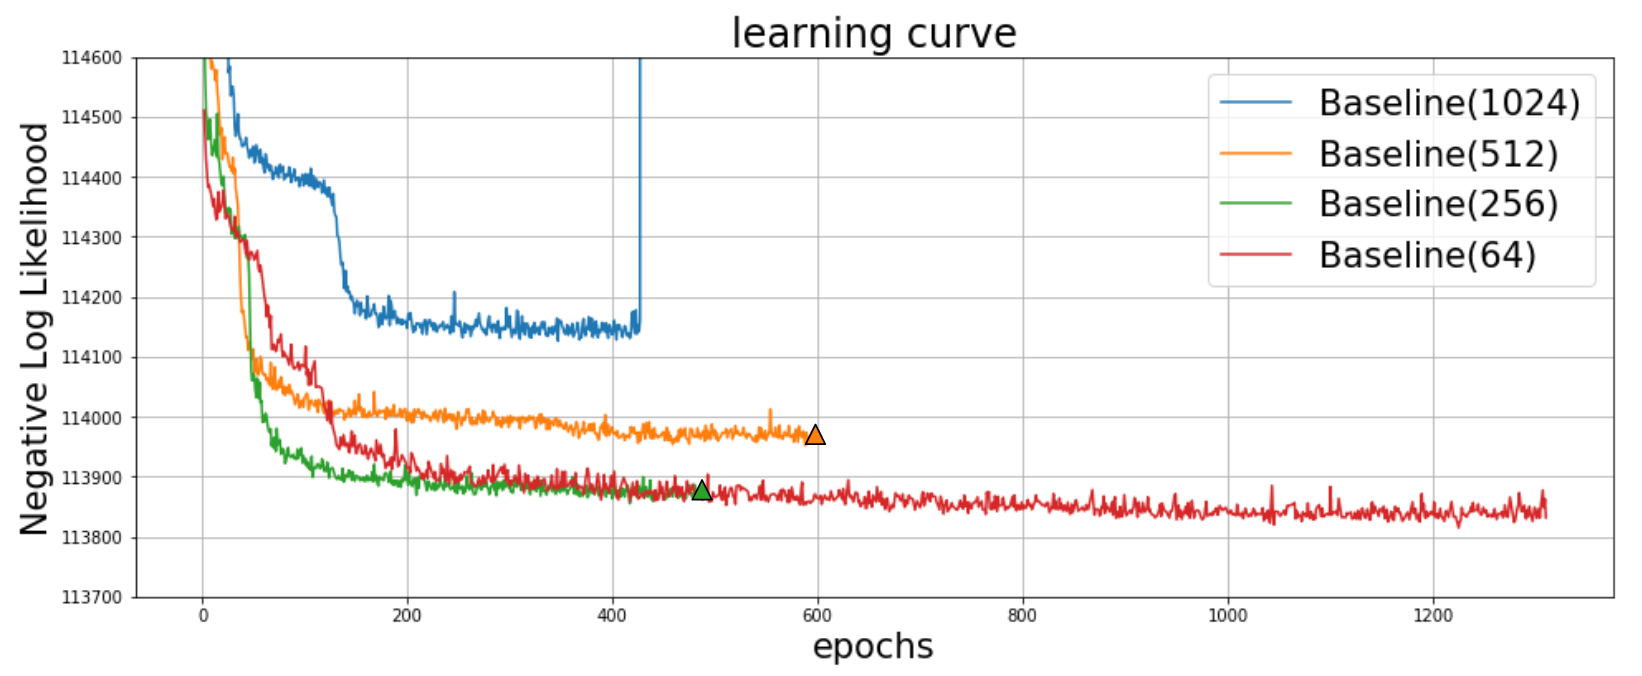
\includegraphics[width=\linewidth]{./figures/dssm_curve_yoko.png}
%     \caption[状態変数の次元を変えた時のDSSMの学習曲線]
%     \label{fig:dssm_curve}
%   \end{center}
% \end{figure}

% ELBOがNanをとったり発散したりすることは数値計算の丸め誤差などの理由も関わるので一旦考えないとしても,明らかに状態変数の次元を大きくすることで精度が下がっていることが図 \ref{fig:dssm_curve}からわかる.

% \subsection{学習が難しくなる理由の考察}
% VAEの学習では前節で述べたような問題は起こらないことを踏まえると,DSSMで学習が難しいのは状態変数の遷移の部分であると考えられる.さらに,状態変数に高次元を仮定したとき,状態変数の遷移の部分では状態変数の生成モデル・推論モデルともに高次元ベクトルから高次元ベクトルへの写像を学習する必要が生じてまずこの部分で学習に時間がかかりやすくなっており,さらに推論モデルが十分に学習されないまま状態変数の事前分布と事後分布のカルバックライブラー距離の最小化が図られてしまうので,学習が安定しにくなっていると考えられる.

% このことから,単に状態変数を高次元にすることはDSSMの性質上適切ではなく,DSSMをより複雑な環境を扱う問題にスケールさせるためには他の方法を考える必要がある.以上の予備実験を受け,次章ではシンプルなDSSMの拡張方法を提案する.

\section{状態表現の階層性を考慮することによる\\深層状態空間モデルの拡張}
\label{chap:proposal}
状態変数の次元を大きくすると,状態変数の遷移の部分で高次元ベクトルから高次元ベクトルへの変換を学習する必要が生じて全体の学習が困難になる.そこで高次元の状態表現の学習時に小さい状態変数で学習した各時刻の状態表現を補助的に用いることを考え,図\ref{fig:proposal}のグラフィカルモデルで表されるDSSMの拡張モデルを提案する.またこのモデルの学習アルゴリズムをアルゴリズム\ref{alg1}に示す.

% \caption[hoge]{fuga}
\begin{figure}[h]
  \begin{center}
    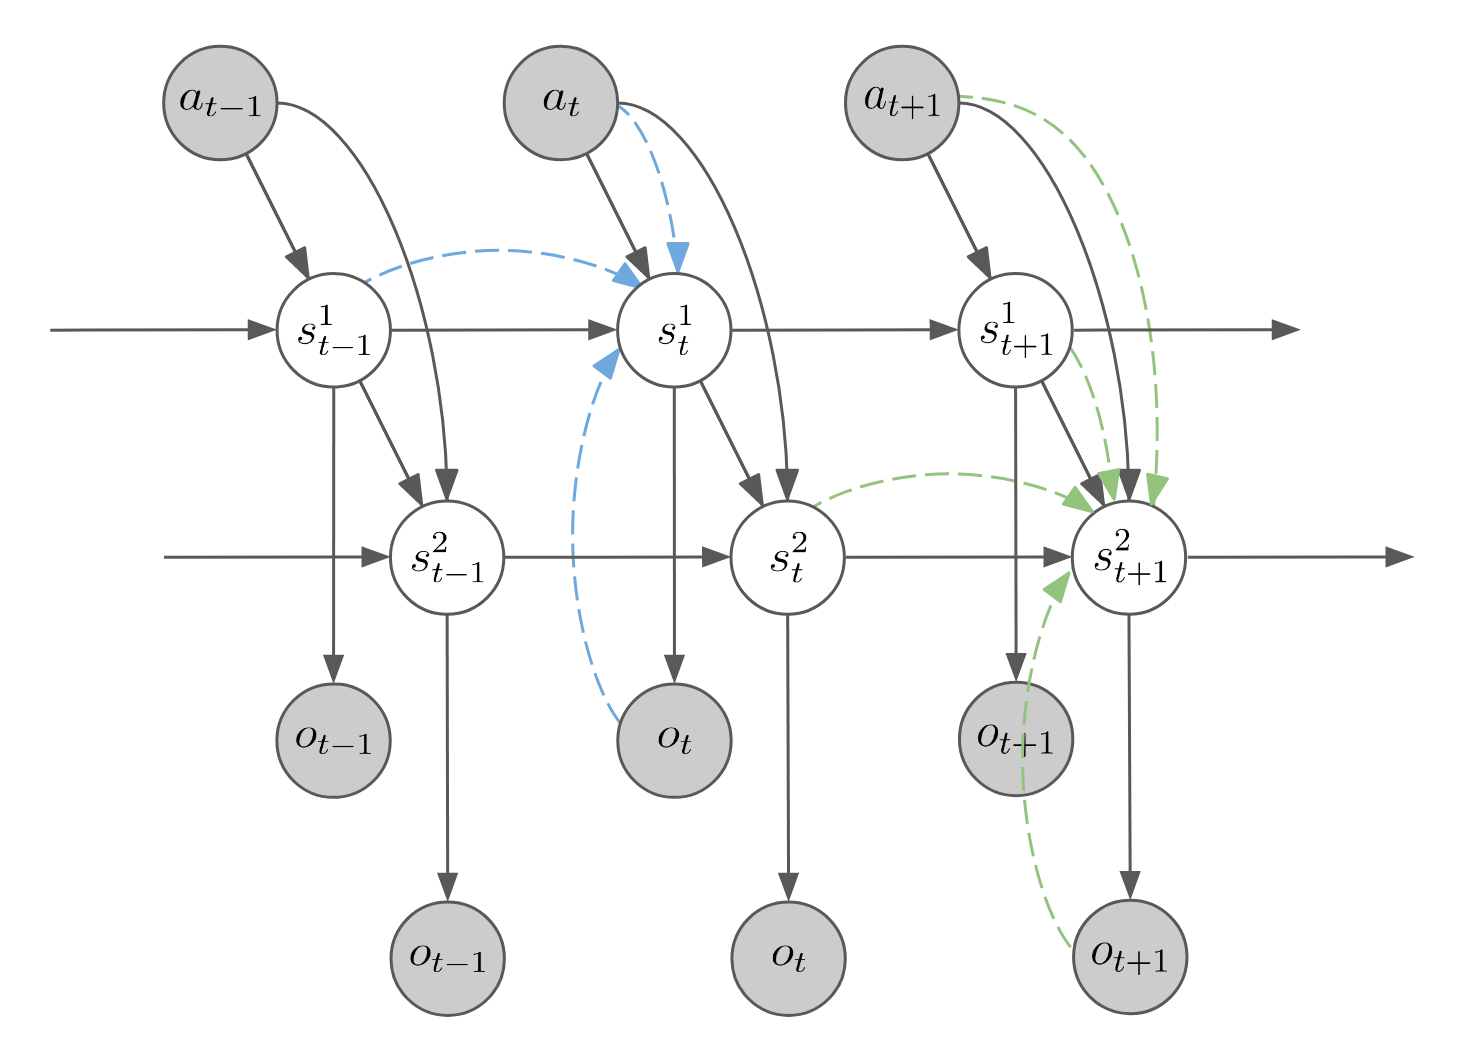
\includegraphics[width=\linewidth]{./figures/proposal_train.png}
    \caption[提案手法(二階層)のグラフィカルモデル]{\small 提案手法のグラフィカルモデル.実線が生成分布,点線が推論分布を示す.$s^1$, $s^2$の推論分布は簡単のため時刻t, t-1でのみ記載している.また2つずつ記載されている$o_t$は同じデータを示すが.異なるsから独立に生成されることを明示している.}
    \label{fig:proposal}
  \end{center}
\end{figure}

% \subsection{確率モデル・最適化}

% ここまでで状態変数の階層性とその遷移を考えたが,この階層性の仮定はDSSMの性能の向上に十分寄与しうると考え,状態変数の階層性を帰納バイアスとしてDSSMに組み込み以下のようなモデルとその最適化アルゴリズムを提案する.

% \vspace{\baselineskip}
% 提案手法のグラフィカルモデルを図(\ref{fig:proposal})に示す.提案手法は,DSSMの状態変数をN層に階層化したモデルである.図(\ref{fig:proposal})は2階層の提案モデルを表している.図(\ref{fig:proposal})の上側の状態変数から一階層の状態変数・二階層の状態変数と呼ぶことにすると一階層の状態変数が低次元ベクトル,二階層の状態変数が高次元ベクトルになっており,高次元の状態変数の生成・推論時に低次元の状態変数を用いるようなモデルになっている.高次元の状態変数の遷移時に低階層の状態変数を用いて写像先に関する情報を補助的に与えることで,学習を安定化させる効果が期待される.またモデルの評価時には,最高層の観測の生成モデル $p(o_t|s^N_t)$ を用いる.

\begin{algorithm}[h]               
  \caption{\small N階層DSSMの学習アルゴリズム}
  \label{alg1}
  \begin{algorithmic}
    \REQUIRE \small 階層数 $N$ 
    \FOR{i = 1 to $N$}
      \WHILE{\small $i$ 階層の学習が収束していない}
        \STATE \small $1 \sim i-1$階層のパラメータを固定し, 
        \STATE \small $i$階層を次の目的関数$L$で学習する
        \STATE $\hspace{1em} L(a_{1:T}, o_{1:T}) = \sum_{t=1}^T ( {L^i}_{reconst} - {L^i}_{KL}) $
        \STATE where, 
        \STATE $\hspace{1em} {L^i}_{reconst} = \mathbb{E}_{s^i_t} [\log p(o_t|s^i_t)]$
        \STATE $\hspace{1em} {L^i}_{KL} = \mathbb{E}_{s^i_{t-1}} [\mathrm{D_{KL}}(q(s^i_t|s^i_{t-1}, a_t, o_t) \| $
        \STATE $\hspace{9em} p(s^i_t|s^i_{t-1}, a_t, o_t, s^{i-1}_t))] )$
      \ENDWHILE
    \ENDFOR
  \end{algorithmic}
\end{algorithm}

% \small
% \begin{eqnarray}
%   &&L(a_{1:T}, o_{1:T}) = \nonumber \\
%   &&\hspace{1em}\sum_{t=1}^T \left( \mathbb{E}_{s^i_t} [\log p(o_t|s^i_t)] \hspace{18em} \right. \nonumber \\
%   &&\hspace{1em}\left. - \mathbb{E}_{s^i_{t-1}} [\mathrm{D_{KL}}(q(s^i_t|s^i_{t-1}, a_t, o_t) \| p(s^i_t|s^i_{t-1}, a_t, o_t, s^{i-1}_t))] \right) \nonumber \\ 
%   \label{eq:proposal}
% \end{eqnarray}
% \normalsize


% \small
% \begin{eqnarray}
%   &&\hspace{1em}L(a_{1:T}, o_{1:T}) = \sum_{t=1}^T ( L_{reconst} + L_{KL}) \hspace{3em} \nonumber \\
%   &&where, \nonumber \\
%   &&\hspace{1em}L_{reconst} = \mathbb{E}_{s^i_t} [\log p(o_t|s^i_t)] \nonumber \\
%   &&\hspace{1em}L_{KL} = - \mathbb{E}_{s^i_{t-1}} [\mathrm{D_{KL}}(q(s^i_t|s^i_{t-1}, a_t, o_t) \| p(s^i_t|s^i_{t-1}, a_t, o_t, s^{i-1}_t))]
%   \label{eq:proposal}
% \end{eqnarray}
% \normalsize

% \vspace{\baselineskip}
% 次に提案手法の学習アルゴリズムをアルゴリズム\ref{alg1}に示す.この学習アルゴリズムは前節「階層的な状態表現の遷移」で述べた,習熟度に合わせて徐々に高次元の状態ベクトルの遷移を学習するという考え方に基づいており,これにより安定した学習が見込める.今回簡単のために高階層の潜在表現の学習時にはそれより低階層の状態表現の学習を止めているが,他の方法も考えられ,これついては考察「低次元状態ベクトルの階層の再学習」で述べる.

\section{実験}
\label{chap:experiment}
% 第4章で述べた提案手法の有効性を検証するために,BAIR Push Dataset\cite{ebert2017selfsupervised}という行動条件付き映像予測用のデータセットを用いて評価実験を行った.本章では実験の内容について説明した後に実験結果について述べる.


\subsection{実験内容}

提案手法とベースラインの比較実験を行う.提案手法は64次元と512次元の二階層の状態ベクトルを持つモデルと,64次元と512次元と1024次元の三階層の状態ベクトルを持つモデルで実験を行った.ベースラインと提案手法の実装の差は必要最小限にとどめ,どちらも学習時には10フレーム先までの予測を行った.

% \subsubsection{データセット}

% 今回用いるBAIR Push Dataset\cite{ebert2017selfsupervised}は行動条件付き映像予測と行動条件をつけない映像予測のどちらの研究でも用いられるデータセットであり,カリフォルニア大学バークレー校によって制作・公開されている.
% こちらのデータセットは,様々な物体がおかれた机の上をロボットアームがランダムに掻き乱すようにして様々なデータが記録されており,今回はその中から行動系列$\vec{a}$と固定視点から観測された画像系列$\vec{o}$を用いる.今回用いる行動系列$\vec{a}$は,具体的にはロボットのエンドエフェクタの位置姿勢の命令値になっている.観測画像は64x64サイズのRGB画像で,これらのデータは10hzで撮られている.また訓練時と評価時に使われる物体は揃えられている.

% \subsection{提案手法の実装}
% 提案手法はベースラインの節で説明した部分モデルをほぼそのまま用いる.二階層目以上の第i層では,各遷移モデルの入力として一時刻前の状態変数$s^i_{t-1}$と行動$a_t$だけでなく,一つ低次元の層の同じ時刻の状態ベクトル$s^{i-1}_t$も入力とする.また,提案手法では,パラメータを固定している層の状態ベクトルのサンプリングには,モデルの評価時の設定に合わせて常に事前分布を用いている.これは,パラメータを固定している層はそれ以上学習されないために,事前分布より良い表現が下の階層に渡されることはなく,むしろ事前分布で足りない表現を積極的に下の階層の学習で獲得できるようにするためである.
% その他はベースラインの実装と変えていない.


\subsection{実験結果}

% 簡単のため,ここから状態変数の次元を64にしたベースラインモデルを「ベースライン(64)」,状態変数の次元を64と512にした提案手法モデルを「提案手法(64 + 512)」などと呼ぶ.

\begin{figure}[h]
    \begin{center}
        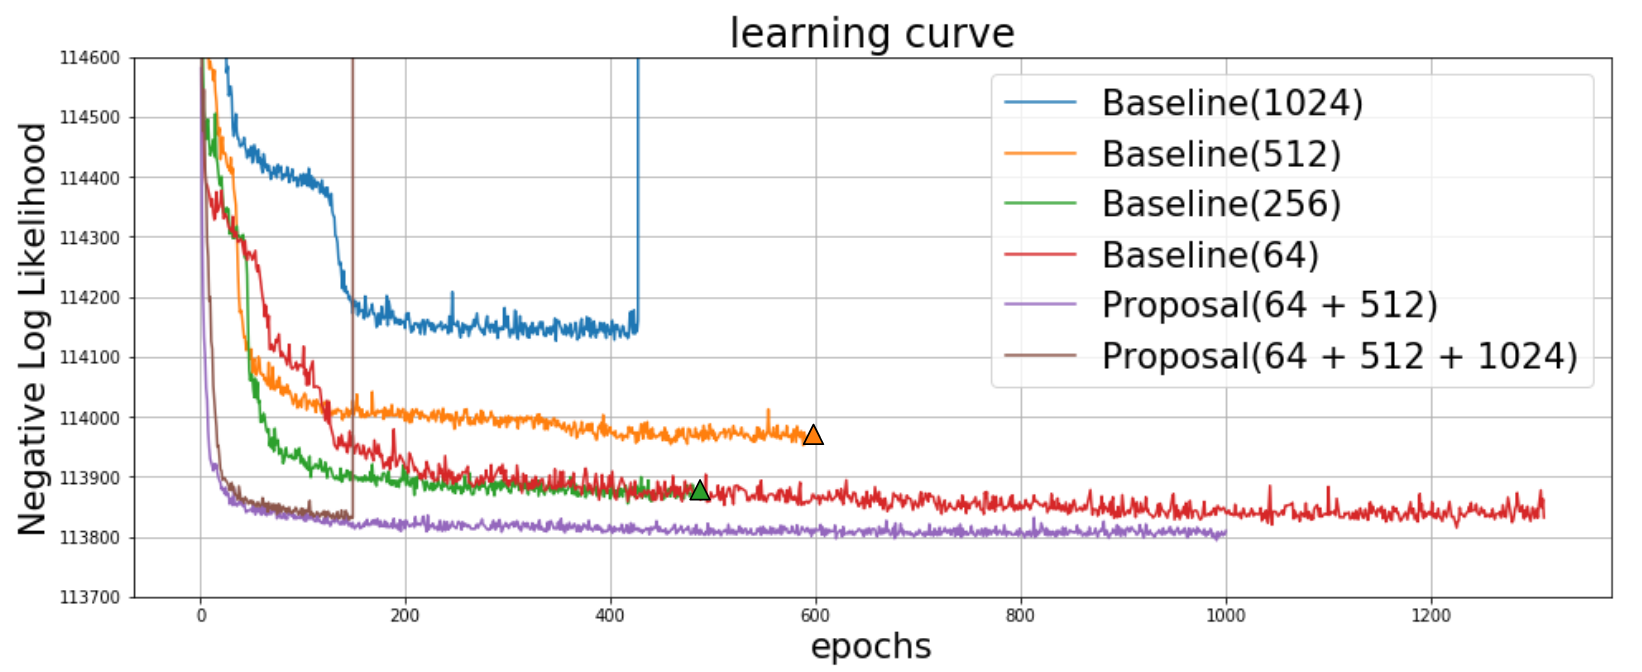
\includegraphics[width=\linewidth]{./figures/curve_yoko.png}
        \caption[提案手法の学習曲線]{\small ベースラインと提案手法の学習曲線.横軸がepoch数で縦軸が目的関数の値である.グラフ中に三角で示されるのは目的関数の値にNanが出力されてしまったことを示す.Baseline(1024)は400epochを過ぎたあたりで目的関数の値が発散し異常な値をとっている.}
        \label{fig:curve}
    \end{center}
    \end{figure}
\normalsize

\begin{table}[h]
    \begin{center}
    \caption{\small 手法ごとの定量評価指標(尤度)}
    \begin{tabular}{|c||c|} \hline
      \small 手法 & \small 負の対数尤度 \\ \hline \hline
      \small ベースライン(64) & \small $1.1384 \times 10^5 $ \\ \hline
      \small 提案手法(64 + 512) & \small $\bm{1.1381 \times 10^5 }$ \\ \hline
      \small 提案手法(64 + 512 + 1024) & \small $1.1383 \times 10^5$ \\ \hline
    \end{tabular}
    \label{table:evaluation}
    \end{center}
  \end{table}
\normalsize

表(\ref{table:evaluation})に最終的な負の対数尤度を示す.

% まず図(\ref{fig:curve})について,ベースライン(512)と提案手法(64 + 512)との比較から,二階層にすることで潜在変数の次元を512次元と大きくした際にもうまく学習が進むようになったことがわかる.これは,高次元の状態変数の学習時に学習済みの低次元の状態変数の情報を用いることで狙い通り学習が安定したためだと考えられる.次にベースライン(64)と提案手法(64 + 512)の比較から,高次元の潜在変数で学習させたことによってより高い尤度の映像を生成できるようになったことがわかる.これは潜在変数を高次元にした方が多くの情報を保持しやすく,適切に学習が進みさえすれば予測性能が向上しやすくなるためだと考えられる.最後に三階層の提案手法(64 + 512 + 1024)について見ると,ベースライン(1024)と比較し明らかに学習が進んだものの,ベースライン(64 + 512)と比較して精度の改善は見られず,潜在変数の次元を大きくすることだけでは精度の向上には限界があるということが伺える.

% 図(\ref{fig:compare_ad})は評価用データで10フレームの行動条件付き映像予測により生成された映像のサンプルで,正解映像とベースライン(64)による予測映像,提案手法(64 + 512)による予測映像を比較している.どちらのモデルもロボットアームの位置はほぼ正しく予測ができているが,環境中の物体の見た目には差が見られた.図(\ref{fig:pred_a}), 図(\ref{fig:pred_b})を見ると,ベースラインでは環境中の物体の輪郭がぼやけて灰色がかっているのに対し,提案手法では特に物体が密集していない場合に比較的物体一つ一つの生成が鮮明になっていることが見て取れる.これは潜在変数の次元を大きくし保持できる情報を増やすことに成功したためだと言える.しかしフレームごとの見た目には改善が見られたものの,物理的な操作についての予測はあまり改善が見られなかった.図(\ref{fig:pred_c})では,正解映像ではロボットアームの移動によって中央の緑の物体の姿勢を変えているが,そもそもベースラインではその物体を生成できておらず,提案手法でも僅かに黒っぽい点として表されている程度で姿勢の変化を読み取ることはできない.図(\ref{fig:pred_d})は,正解映像では滑らせるようにして2つの物体を近づけており,提案手法のでは2つの物体の輪郭が見られるが,机の色やロボットアームの色と途中から同化してその動きを追うことは困難である.このように物理的な操作の予測を改善するにはまず一フレーム一フレームの質を上げる必要があると考えられ,今回は物理的な操作の予測の改善はあまり見られなかった.最後に図(\ref{fig:pred_long})は,各モデルで学習時よりも長い30フレームの映像予測をした際の生成映像である.ベースライン・提案手法ともにロボットアームの動きはほぼ正解映像と一致しているが,ベースラインでは右端に映る物体が映像を予測するにつれて青色から緑色に変わってしまっているのに対し,提案手法は背景や周りの物体について一貫性が保たれていた.これは,潜在変数の次元が小さいまま性能をあげようとすると潜在表現に含まれる情報が密になりすぎて遷移時に遷移とは関係のない情報も変化させてしまいやすいという問題がある可能性があり,一方提案手法は高次元の潜在変数を使うためにそのような問題は生じなかったと考えられる.

% また図(\ref{fig:pred_a})では,水色の物体の予測位置が提案手法が生成した映像と正解映像とで少しずつずれているが,このことから画像を一画素ずつ潜在表現で記憶しているのではなく,物体の見た目と位置を別々に保存するように学習がすすんでいたことが伺える.

% 高次元で学習できるようになった.これは深層状態空間モデルの大きな問題点を克服できたと言える.

\begin{figure}[tp]
    \centering
    \subfloat[改善が見られた例]{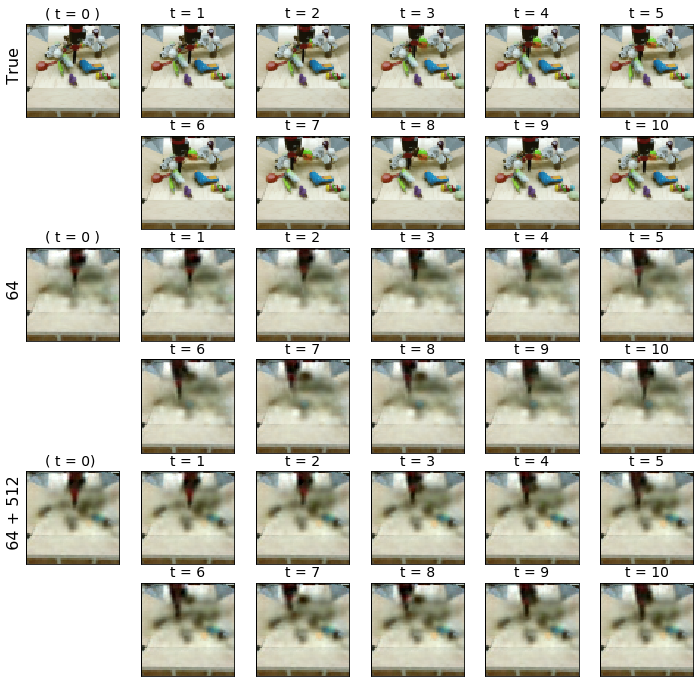
\includegraphics[clip, width=0.75\linewidth]{./figures/pred_a.png}
    \label{fig:pred_a}}
    \\
    \subfloat[改善が見られなかった例]{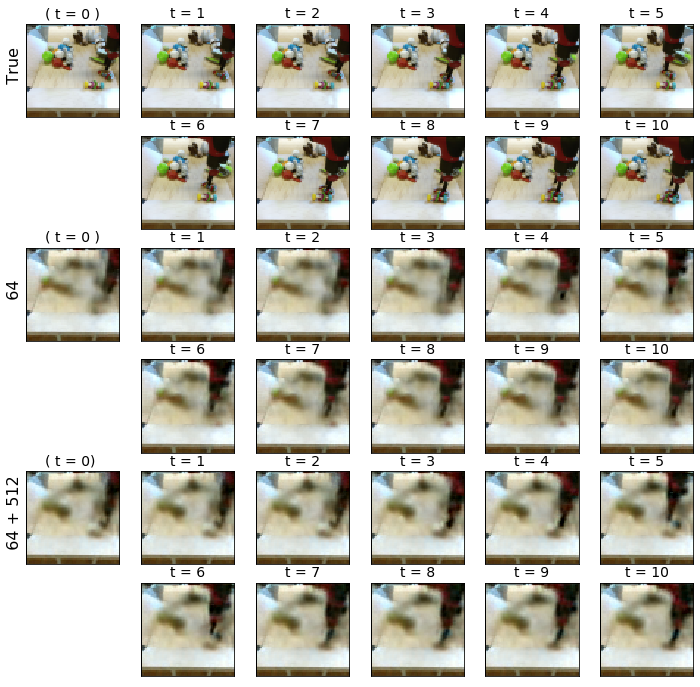
\includegraphics[clip, width=0.75\linewidth]{./figures/pred_d.png}
    \label{fig:pred_d}}
    \caption[映像予測結果1]{\small 映像予測結果1.「True」が正解映像,「64」がベースライン(64)での予測結果,「64 + 512」が提案手法(64 + 512)での予測結果を示す.また$t = 0$は初期状態の推論時に与えられるフレームを示す.}
    \label{fig:compare_ad}
\end{figure}

\section{考察}
課題メイン

\section{結論}

本論文では,実機ロボットへの応用を見据えて深層状態空間モデルを用いた映像予測について取り上げた.まず深層強化学習などで用いられているシンプルな深層状態空間モデルでは複雑な環境を扱う問題設定に上手くスケールしない問題を示し,その上で深層状態空間モデルの状態表現の階層性を明示的にモデル化した提案手法によってより高次元の状態表現を扱えるようにし,さらに映像予測の性能が向上することを示した.
実験では,定性的な大きな優位性は示せなかったものの,高次元の状態変数を用いた学習を可能にしたことは深層状態空間モデルの大きな問題を克服したと言える.これにより,これまで映像予測の分野では実機ロボットへの応用上の制約が多いにも関わらず自己回帰的なモデルの研究が主流であったが,状態空間モデルベースの手法が見直されるきっかけになるかもしれない.

第六章では展望として深層状態空間モデルの研究の方向性を複数上げたが,これらの研究をすすめることによってより高性能な予測が可能になり,また実機への応用の可能性も高められると考える.さらに社会応用の例として,映像予測の実機応用に加え,新たな物理シミュレーションの近似アプローチと新たなロボット学習のあり方の可能性について述べた.この二つの応用例は現段階では可能性の話に過ぎず実現可能かは定かでないがどちらも実現すれば社会的な価値は大きいと考えられるので,今後も慎重に研究を継続していきたい.

\bibliography{references}
\bibliographystyle{unsrt}
%%%%%%%%%%%%%%%%%%%%%%%%%%%%%%%%%%%%%%%%%%%%%%%%%%
\end{document}